\section{Step 4 - Time for Practice}
\subsection{Extending our sample}
The last sample of the former section is now used as a starting point for getting some practice.

Did you notice the little coordinate cross at the bottom of the screen? 
It shows you the $x$-, $y$- and $z$-direction in the displayed space.
To get some practice we place a larger coordinate cross at the origin.
Execute {\tt Step4\_1.py}, click on menu {\tt Draw} menu-item  {\tt draw coordinates} to get the screen shown in figure~\ref{STEP_4_1_SCREEN}.
% +++++++++++++++++++++++++++++++++++++++++++++++++++++++++++++++++++++++ 
% +++ Bild: Step 4_1 ++++++++++++++++++++++++++++++++++++++++++++++++++++
% +++++++++++++++++++++++++++++++++++++++++++++++++++++++++++++++++++++++ 
\begin{figure}[h]
\begin{center}
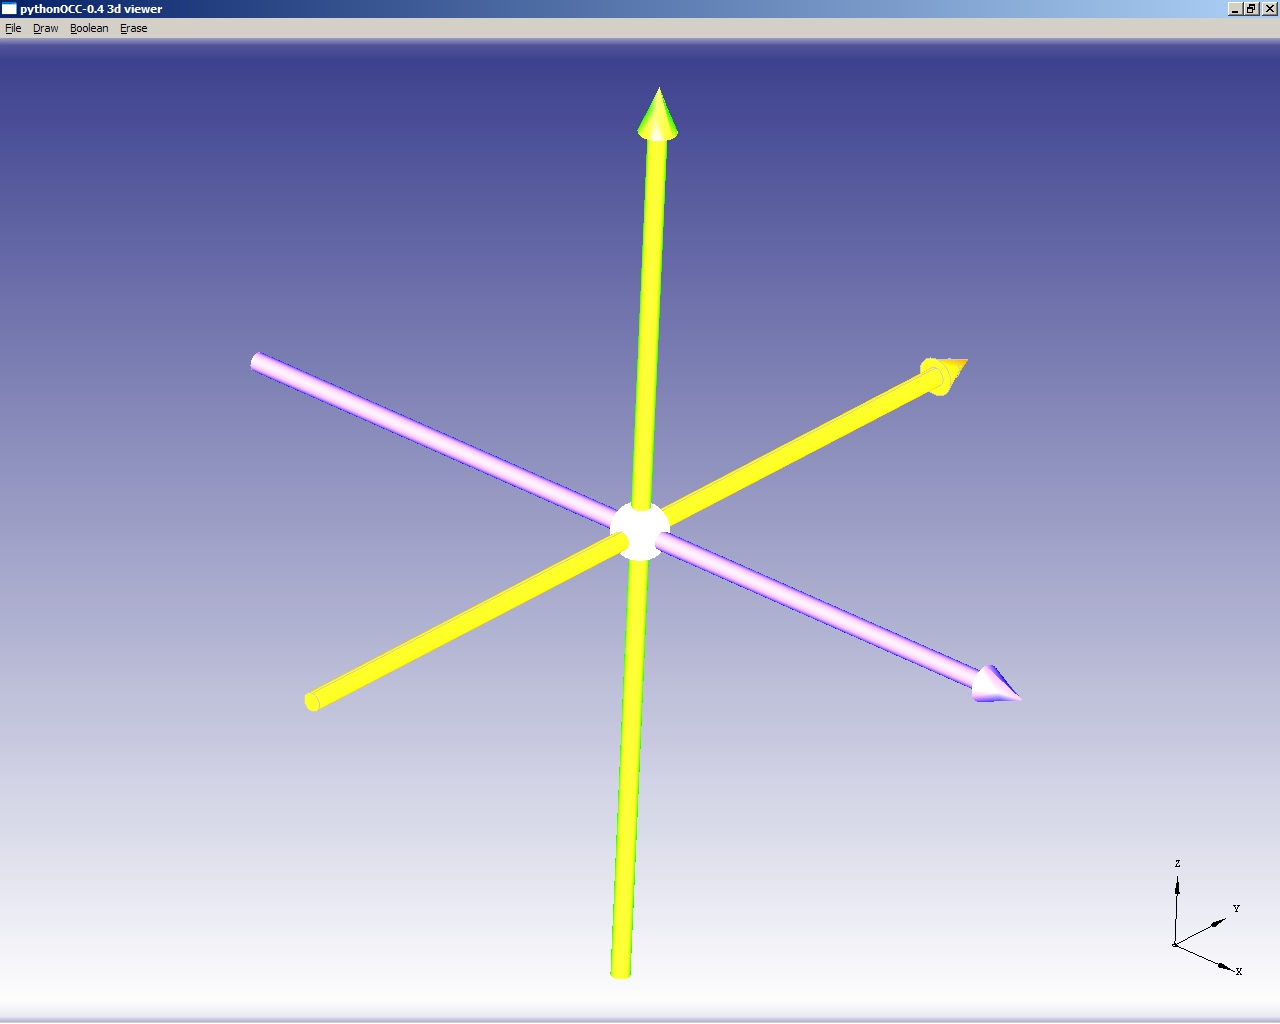
\includegraphics[height=8.5cm,width=11.3cm]{Step4_1.jpg}
\end{center}
\caption[Screenshot of Step4\_1]{\label{STEP_4_1_SCREEN}Screenshot of Step4\_1}
\end{figure}

To see how this is done start reading Listing~\ref{LISTING_STEP4_1_PY_A} where the function which is called after selecting that menu item is presented.
The function is heavily commented and should be understood without difficulty.
%
\begin{python}[moreemph={[4], 46, 48},caption={Step4\_1.py - Drawing a larger, coloured coordinate system -- function {\tt draw\_coordinates} which is called by clicking on the menu},label=LISTING_STEP4_1_PY_A]
def draw_coordinates(event=None):
    # The radius of a sphere at the origin
    centerpoint_sphere_radius = 30.0
    # The length of every axis starting at -length/2 and ending at length/2
    arrowlength = 1000.0
    # Radius of the arrow shaft of every axis
    radius_of_arrow_shaft = 10.0
    # Length of every axis
    lenght_of_arrow_head = 50.0
    # Radius of the arrow heads cone
    radius_of_arrow_head = 20.0
    # Create the Coordinate and Draw it
    CoordinateCrossShape(   centerpoint_sphere_radius,
                            arrowlength,
                            radius_of_arrow_shaft,
                            lenght_of_arrow_head,
                            radius_of_arrow_head )
\end{python}

Function {\tt draw\_coordinates} calls {\tt CoordinateCrossShape}.
We should also have a look at that function given in Listing~\ref{LISTING_STEP4_1_PY_B}.
Before you start reading the code let me state that all the functionality used in that function was already explained in the last section.
I also like to mention that the different parts of the coordinate cross are not combined by Boolean functions.
On one hand this makes it easy to apply different colours to the single parts on the other there is no need to move or turn the coordinate axis - these are our world coordinates.
Finally I would like to guide your attention at the end of the function.
It does not return anything.
The function itself draws the coordinate cross.
%
\begin{python}[moreemph={[4], 46, 48},caption={Step4\_1.py - Drawing a coordinate system -- function {\tt CoordinateCrossShape} which is called by function {\tt draw\_coordinates}},label=LISTING_STEP4_1_PY_B]
def CoordinateCrossShape(   centerpoint_sphere_radius,
                            arrowlength,
                            radius_of_arrow_shaft,
                            lenght_of_arrow_head,
                            radius_of_arrow_head ):
    '''
    Function arrowshape creates the shape of an arrow starting at vector
    pointing into diretcion. We create a cylinder and a cone and combine the 
    utilising OCC.BRepAlgoAPI.BRepAlgoAPI_Fuse.

    @param vector: starting point of the arrow
    @type  vector: scipy array(3,1)
    @param directionvector: direction of the arrow
    @type  directionvector: scipy  array(3,1)
    @param arrowlength: length of the arrow
    @type  arrowlength: scalar
    @param radius_of_arrow_shaft: radius of the arrow shaft
    @type  radius_of_arrow_shaft: scalar
    @param lenght_of_arrow_head: length of the arrow head
    @type  lenght_of_arrow_head: scalar
    @param radius_of_arrow_head: radius of the arrow head
    @type  radius_of_arrow_head: scalar
    @return: Arrow as Shape object
    '''
    # The origin of the coordinate system
    Origin = scipy.zeros((3,1),dtype=float)
    # The direction unit vectors of the axis
    xDir = scipy.zeros((3,1),dtype=float)
    xDir[0,0] = 1.0
    yDir = scipy.zeros((3,1),dtype=float)
    yDir[1,0] = 1.0
    zDir = scipy.zeros((3,1),dtype=float)
    zDir[2,0] = 1.0
    
    # Create the center point sphere shape at the origin
    OriginSphere = sphere_from_vector_and_radius(   Origin, 
                                                    centerpoint_sphere_radius )
    OriginSphereShape = OriginSphere.Shape()

    # Create the XAxis shape
    XAxisShape = arrowShape(    Origin - 0.5 * arrowlength * xDir, 
                                xDir,
                                arrowlength,
                                radius_of_arrow_shaft,
                                lenght_of_arrow_head,
                                radius_of_arrow_head )
    # Create the YAxis shape
    YAxisShape = arrowShape(    Origin - 0.5 * arrowlength * yDir, 
                                yDir,
                                arrowlength,
                                radius_of_arrow_shaft,
                                lenght_of_arrow_head,
                                radius_of_arrow_head )
    # Create the ZAxis shape
    ZAxisShape = arrowShape(    Origin - 0.5 * arrowlength * zDir, 
                                zDir,
                                arrowlength,
                                radius_of_arrow_shaft,
                                lenght_of_arrow_head,
                                radius_of_arrow_head )
    
    # Display these shapes
    display.DisplayColoredShape( OriginSphereShape , 'WHITE' ) 
    display.DisplayColoredShape( XAxisShape , 'BLUE' ) 
    display.DisplayColoredShape( YAxisShape , 'ORANGE' ) 
    display.DisplayColoredShape( ZAxisShape , 'GREEN' ) 
\end{python}

Why is it possible to draw on the display without receiving it as a parameter?
The reason is that the display is created outside of a class or function.
Look at the end of {\tt Step4\_1.py} which is shown in  Listing~\ref{LISTING_STEP4_1_PY_C}.
%
\begin{python}[moreemph={[4], 46, 48},caption={Step4\_1.py - Creating the display},label=LISTING_STEP4_1_PY_C]
if __name__ == '__main__':
    # OCC.Display.SimpleGuiinit_display() returns multiple
    # values which are assigned here
    display, start_display, add_menu, add_function_to_menu = \
        OCC.Display.SimpleGui.init_display()
...
    start_display()
\end{python}

\subsection{Time for Housekeeping}
Our sample became pretty large.
So lets divide it into two parts:
\begin{description}
\item [{\tt Step4\_2.py}] the main program and
\item [{\tt Step4\_2\_A.py}] a module containing the Scipy stuff and the construction of geometric objects.
\end{description}
Run program {\tt Step4\_2.py} and see that it works exactly like {\tt Step4\_1.py}.
Sure you know how this division works.
We simply took some functions from {\tt Step4\_1.py} and put these into a module called {\tt Step4\_2\_A.py}.
The remaining main script is called {\tt Step4\_2.py}.
In order to tell Python where to look for the outsourced functions we add
\begin{python}
...    
from Step4_2_A import *
...    
\end{python}
at the beginning of {\tt Step4\_2.py}.
Now have a closer look at {\tt Step4\_2\_A.py}.
See that we also modified function {\tt CoordinateCrossShape}.
Look at the function definition we added one parameter. 
It is the parameter {\tt display}.
\begin{python}
def CoordinateCrossShape(   display, 
                            centerpoint_sphere_radius,
                            arrowlength,
                            radius_of_arrow_shaft,
                            lenght_of_arrow_head,
                            radius_of_arrow_head ):
...    
\end{python}
You should also notice that the function call which is done from {\tt Step4\_2.py} uses that additional parameter too.
Of course, we need a structure of parameters which reflects the parameter line of the function called.
\begin{python}
...    
    # Create the Coordinate and Draw it
    CoordinateCrossShape(   display, 
                            centerpoint_sphere_radius,
                            arrowlength,
                            radius_of_arrow_shaft,
                            lenght_of_arrow_head,
                            radius_of_arrow_head )
...    
\end{python}
Why do we have to do that?
Think about a painter painting for some client.
If the client and the painter are in the same room they can point on the canvas to be painted easily.
If these two, the painter and the client, are talking via a phone line and the painter is not in the clients room containing the canvas the client needs to specify his canvas so the painter knows on where to go and paint on.
Note that the painter probably has different clients all of them have their own canvas in their room and all of them may ask the painter to come around and paint on their canvas.
The same is true here. 

\subsection{Once more: Extending the sample}
In this section only a few thing to learn were introduced so far.
Hence we should have a brief look at something not mentioned until now.

We already saw that we can write code like 
\begin{python}
...    
    display.DisplayColoredShape( MyCylinderShape , 'YELLOW' ) 
...    
\end{python}
to draw coloured objects.
What if we like to change other things like material and transparency?
Here the coding gets a little more complicated because we need to be familiar with the {\it Application Interactive Services (AIS)}.
These services are responsible for the presentation including display properties of geometrical structures, display quality, detection and selection.

At the moment I cannot tell how all this can be done and I need to explore the  {\it Application Interactive Services (AIS)} to see how to make use of them.
Nevertheless I want to tell you my actual knowledge which may help you to get things done if you try to make objects transparent and so on. 

Execute {\tt Step4\_3.py} and choose menu {\tt Draw}, menu item {\tt draw cylinder}.
Probably you cannot see the cylinder without moving away from the scene with the mouse.
As an alternative choose menu {\tt Draw}, menu item {\tt draw coordinates} so all objects are shown.
The same is true if you select menu {\tt Draw}, menu item {\tt draw cone}.
I cannot tell how this can be avoided but I will add the solution in some future revision of this document if I'll find any.
Select also  menu {\tt Draw}, menu item {\tt draw sphere 2}.
See that the cylinder intersects with sphere~2.
The cylinder is transparent and sphere~2 can be seen through the cylinder.
In addition the material of the cone is modified compared to the display in {\tt Step4\_2.py}.
Figure~\ref{STEP_4_3_SCREEN} shows the screen presented after you reproduced the steps above.
% +++++++++++++++++++++++++++++++++++++++++++++++++++++++++++++++++++++++ 
% +++ Bild: Step 4_3 ++++++++++++++++++++++++++++++++++++++++++++++++++++
% +++++++++++++++++++++++++++++++++++++++++++++++++++++++++++++++++++++++ 
\begin{figure}[h]
\begin{center}
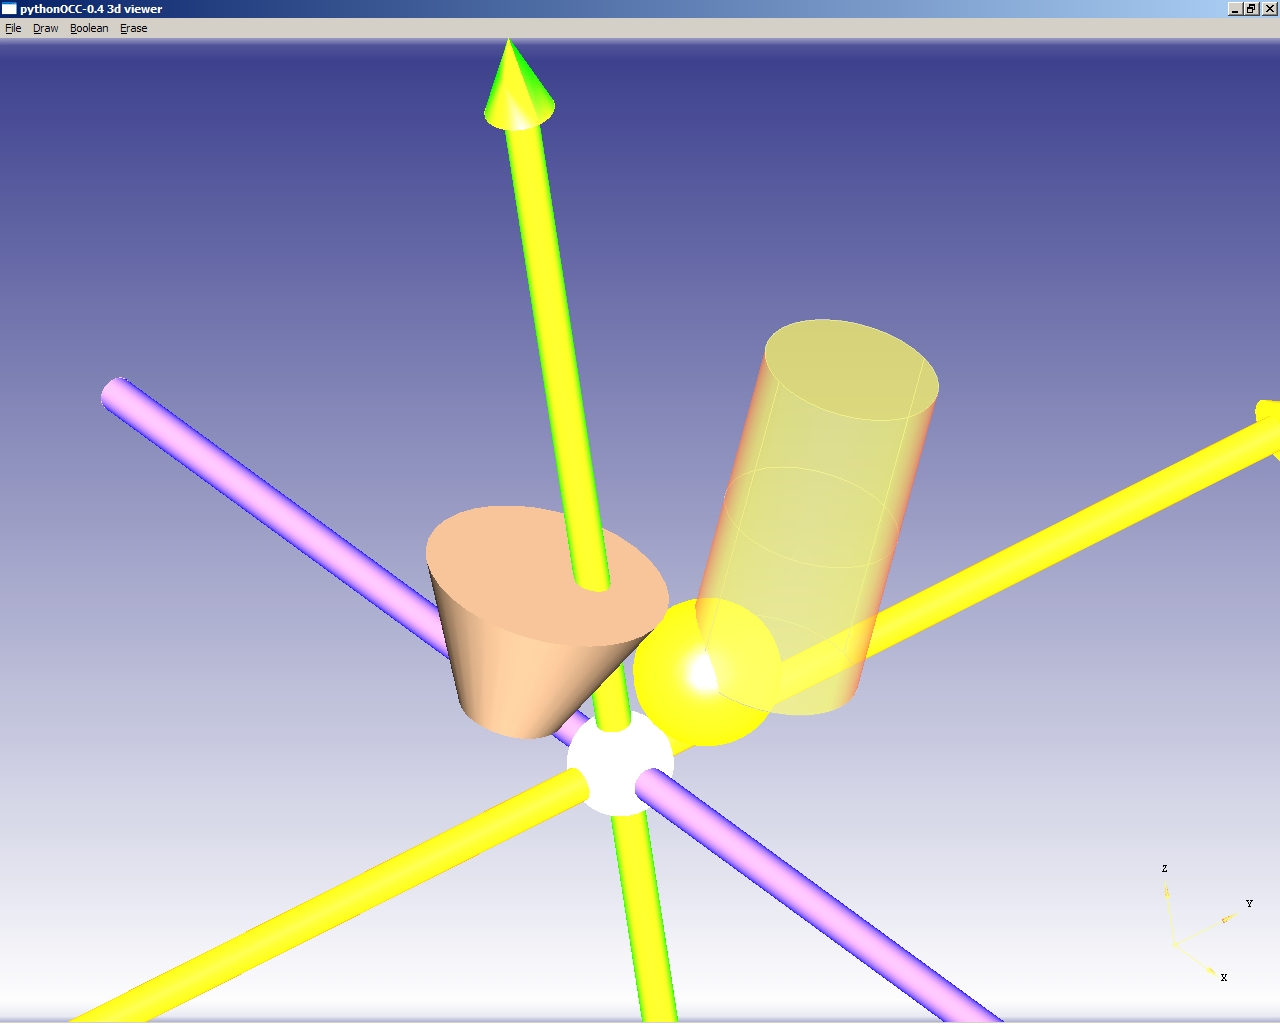
\includegraphics[height=8.5cm,width=11.3cm]{Step4_3.jpg}
\end{center}
\caption[Screenshot of Step4\_3]{\label{STEP_4_3_SCREEN}Screenshot of Step4\_3}
\end{figure}

Listing~\ref{LISTING_STEP4_3_PY} shows the modifications starting at the beginning of {\tt Step4\_3.py} and both, the modified cone and the modified cylinder display.
As already mentioned this sample is not fully understood by me so I only can show how I got it to work.
%
\begin{python}[moreemph={[4], 46, 48},caption={Step4\_1.py - Creating the display},label=LISTING_STEP4_3_PY]
...
from OCC.AIS import *
from OCC.Quantity import *
from OCC.Graphic3d import *
...
def draw_cylinder(event=None):
    # cylinder radius
    Radius = 50.0
    # cylinder length
    Length = 200.0
    # The center point at one of the flat cylinder faces 
    Point = scipy.array([45.0, 80.0, 50.0])
    Point = scipy.reshape(Point,(3,1))
    # The direction of the cylinder from the point given above 
    DirectionFromPoint = scipy.array([25.0, 50.0, 150.0])
    DirectionFromPoint = scipy.reshape(DirectionFromPoint,(3,1))
    # create the cylinder object
    MyCylinder = cylinder_from_point_directionvector_length_and_radius( \
                                                            Point, 
																				DirectionFromPoint,
                                                            Length,
                                                            Radius )
    MyCylinderShape = MyCylinder.Shape()
    
    ais_shape_MyCylinderShape = AIS_Shape( MyCylinderShape ).GetHandle()
    ais_context = display.GetContext().GetObject()
    ais_context.SetColor(  ais_shape_MyCylinderShape,  Quantity_NOC_TOMATO )
    ais_context.SetTransparency( ais_shape_MyCylinderShape, 0.3, True)
    ais_context.Display( ais_shape_MyCylinderShape ) 

def draw_cone(event=None):
    # cone radius 1
    Radius1 = 30.0
    # cone radius 2
    Radius2 = 70.0
    # cone height
    Height = 90.0
    # The center point at one of the flat cone faces 
    Point = scipy.array([-25.0, -50.0, 50.0])
    Point = scipy.reshape(Point,(3,1))
    # The direction of the cone from the point given above 
    DirectionFromPoint = scipy.array([25.0, 50.0, 150.0])
    DirectionFromPoint = scipy.reshape(DirectionFromPoint,(3,1))
    # create the cone object
    MyCone = cone_from_point_height_directionvector_and_two_radii( \
                                                            Point, 
                                                            DirectionFromPoint,
                                                            Height,
                                                            Radius1,
                                                            Radius2 )

    MyConeShape = MyCone.Shape()
    ais_shape_MyConeShape = AIS_Shape( MyConeShape ).GetHandle()
    ais_context = display.GetContext().GetObject()
    ais_context.SetMaterial(    ais_shape_MyConeShape,  
                                Graphic3d.Graphic3d_NOM_STONE )
    ais_context.Display( ais_shape_MyConeShape ) 
\end{python}
